\documentclass[oneside, final, 14pt]{extreport} %односторонняя печать, чистовик, размер текста
\usepackage[utf8]{inputenc} %кодировка
\usepackage[english,russian]{babel} %языки
\usepackage{vmargin} %пакет для регулировки отступов
\setmarginsrb{2cm}{1.5cm}{1cm}{1.5cm}{0pt}{0mm}{0pt}{13mm} %Регулируем отступы
\setpapersize{A4}
\usepackage{indentfirst} %Чтобы первый абзац начинался с отступа
\sloppy %Чтобы текст ни в коем случае не залезал на поля


%Для ссылок
\usepackage{hyperref}

%Вставка рисунка
\usepackage{graphicx}


%код выше не трогаем. Это шапка
\linespread{1.5} % Полуторный интервал


\usepackage{chngcntr} %пакет, чтобы пофиксить нумерацию
\counterwithout{section}{chapter} %отключает учет номера главы при нумерации секций, что позволяет секциям 
%начинаться с 1 вместо 0. 
%\renewcommand{\thesection}{\arabic{section}.0} %Задаём нумерацию в формате number.0

%графика
\usepackage{graphicx}%Вставка картинок правильная
\usepackage{float}%"Плавающие" картинки
\usepackage{wrapfig}%Обтекание фигур (таблиц, картинок и прочего)


\usepackage{ulem} % Для зачёркнутого текста


%для кода
\usepackage{listings}
\usepackage[T2A,T1]{fontenc}
\usepackage[utf8]{inputenc}

\usepackage{listings}

\renewcommand{\contentsname}{Содержание} %Переименуем Оглавление в Содержание

%\setcounter{tocdepth}{3} %Чтобы subsubsection была видна в оглавлении


%Чтобы в списке литературы было написано "Источники", а не Литература
%\addto\captionsrussian{\renewcommand{\bibname}{Источники}}
\addto\captionsrussian{\renewcommand{\contentsname}{\textit{Содержание}}}


\title{Справочная информация по системе Linux}
\author{Алексей Полухин}
\date{2023}


\begin{document}

\begin{titlepage}
    \maketitle
\end{titlepage}


\tableofcontents %Содержание
\newpage

\section*{Предисловие}
Когда я пришёл на свою первую работу в IT, я столкнулся с тем, что мне 
сильно не хватает знания \textit{GNU/Linux}. Два месяца спустя после начала
мне пришлось активно подтягивать свои знания по этой теме. 

Изначально я писал этот конспект, чтобы лучше запомнить информацию и чтобы всегда иметь 
под рукой справочный файл с самыми необходимыми данными. Но потом я решил выложить этот документ
в открытый доступ, чтобы все начинающие специалисты могли использовать этот замечательный конспект.

Так как я записывал по большей части только то, что для меня было новым и интересным, здесь может не быть описания 
некоторых совсем простых вещей, (таких как команды \textit{cd, ls, mv, cp, rm \dots}).

Внести вклад в проект или найти более свежую версию конспекта можно на странице https://github.com/besthedgehog/linux



\vspace*{\baselineskip}

\begin{flushright}
    Успехов в освоении Linux! 

    \vspace*{\baselineskip}

    \textit{Алексей Полухин}
\end{flushright}

\newpage

\begin{figure}[ht]
    \centering
    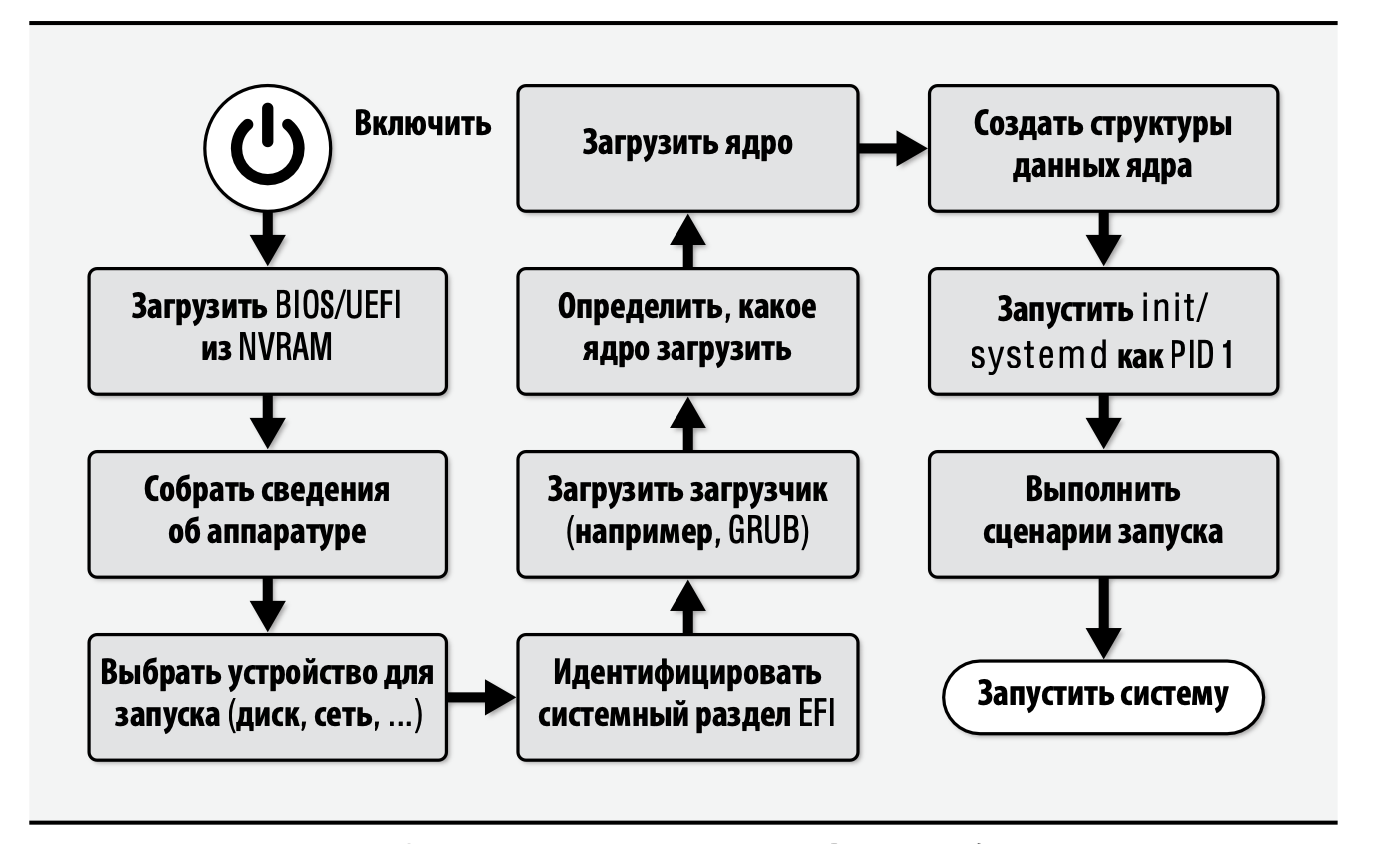
\includegraphics[width=0.9\textwidth]{1.png}
    \caption{Процессы загрузки Linux и Unix}
    \label{fig:1}
\end{figure}

\section{Справочная информация. Полезные сведения}


\textbf{Демон в Linux (служебный пользователь)} --- \textit{фоновый процесс}. Программа на уровне пользователя

Информация о пользователях содержится в файла /etc/passwd. Данные хранятся в следующем порядке: (имя, x, UID, группа, коммент, дом\_каталог, командная\_оболочка\_пользователя)

Информация о группах содержится в файле /etc/group. (имя группы, индентификатор группы, кто входит)

Информация о паролях содержится в файле /etc/shadow (там хранится хэш)

\textit{Хеш-функция} --- такая функция, что при известном $ y = f(x) $ невозможно восстановить $x$.
Пример $ y = x^{2}$. (Ещё примеры: $y = sign(x)$, $y = cos(x)$, функция Дирихле). Однозначно восстановить $x $ невозможно. То есть это функция с неоднозначным соответствием.
Так же хеш (результат работы функции) всегда одной и той же длины.

\textit{аутентификация} --- проверка наличия такого пользователя (совпадение логина и пароля)

\textit{авторизация} --- проверка прав доступа к серверу (уже после корректоного совпадения логина и пароля)

Система Linux не хранит пароли. Только хеши паролей. То есть после ввода пароля рассчитывается хеш и, совпадении хранимого и рассчитанного хешей выполняется вход.


Права досутпа к файлам с системе Linux рассмотрены на Рис.~\ref{fig:7}.
\begin{figure}[ht]
    \centering
    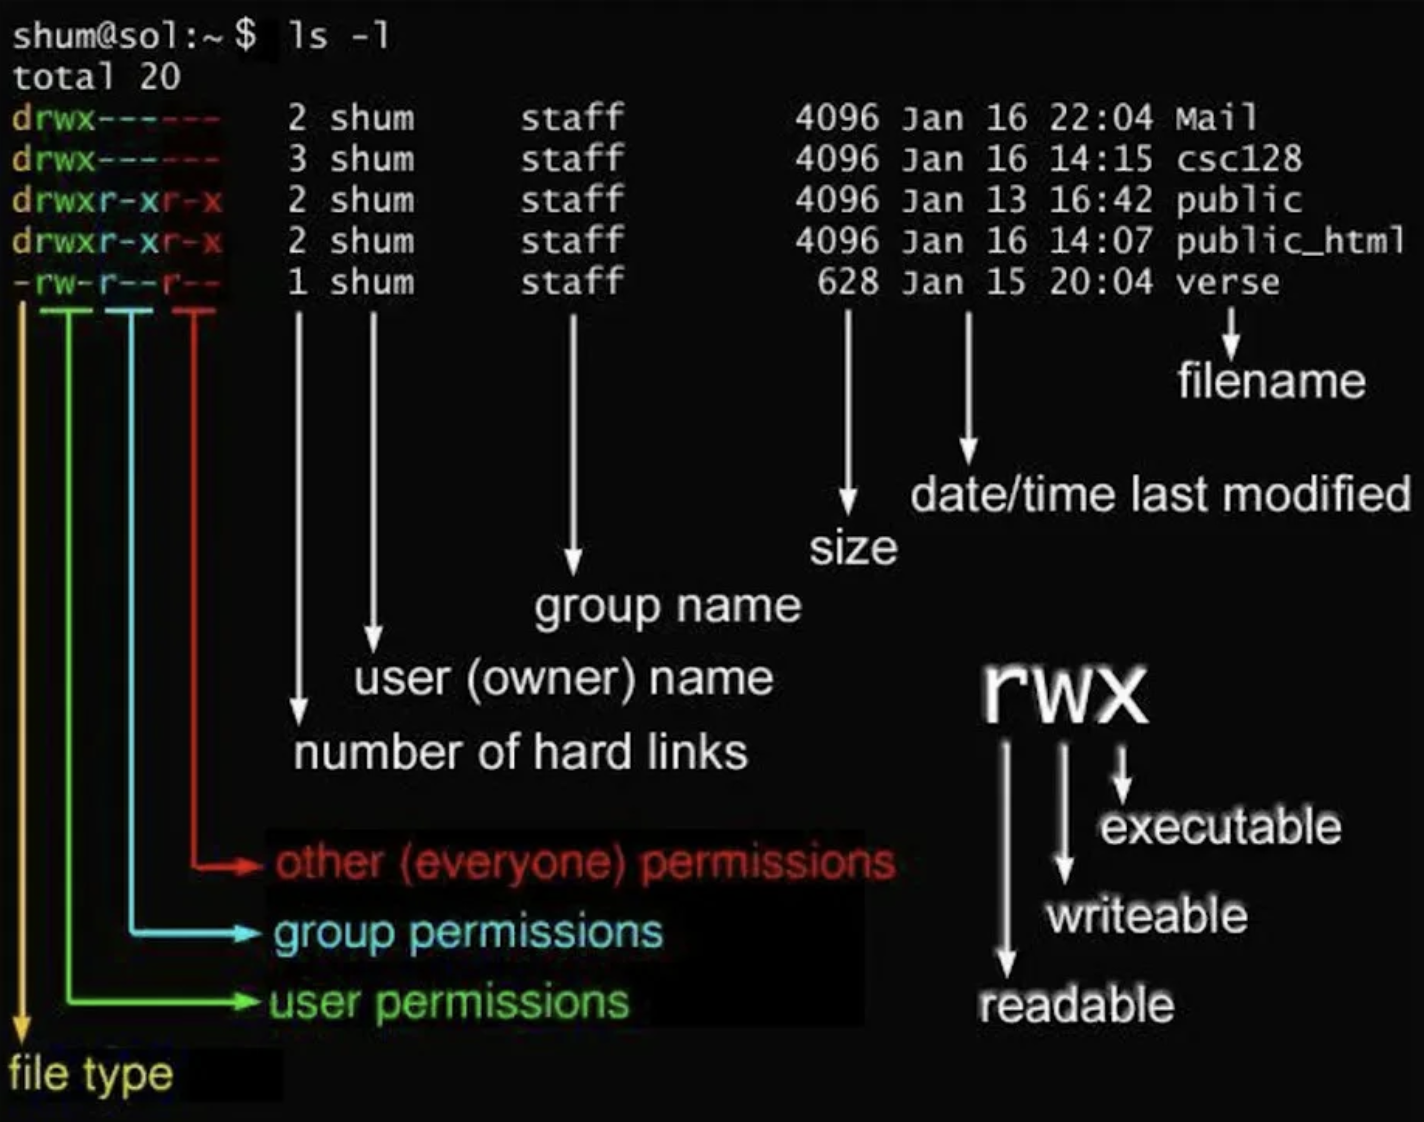
\includegraphics[width=0.9\textwidth]{7.png}
    \caption{Права доступа к файлам}
    \label{fig:7}
\end{figure}

Так же права доступа можно задавать, использую восьмиричную систему (Таблица~\ref{table:1}).
Сумма чисел из таблицы даёт права. То есть 761 означает, что владелец файла обладает всеми 
правами, группа владельца обладает правами на чтение и запись, остальные обладают только 
правом \sout{хранить молчание} на исполнение.



\begin{table}[h]
    \centering
    \begin{tabular}{|c|c|}
    \hline
    Права & Восьмиричное представление\\ 
    \hline
    Read (Чтение) & 4 \\ 
    \hline
    Write (Запись) & 2 \\
    \hline
    Execute (Выполнение) & 1 \\
    \hline
    \end{tabular}
    \caption{Права доступа к системе}
    \label{table:1}
\end{table}

\textit{Интересно,} что право \textit{x} для директории, означает, что мы можем зайти в директорию 
с помощью команды cd. А право \textit{r} означает, что мы можем прочитать содержимое директории (с 
помощью команды ls -l).



\textbf{Переменная окружения} --- это специальные переменные, которые использует система для
облегчения своих настроек со стороны пользователя (начинаются с символа \$) 

\$HISTSIZE --- размер истории команд \textit{bash}

\$ echo \$HISTSIZE 

1000

\vspace{\baselineskip}

Ещё полезная переменная \$PATH --- каталоги, в которых командная оболочка 
будет искать исполняемый файл. (если в них положить свой \textit{script} на bash,
то потом можно просто вводить команду \textit{script} в терминал и скрипт будет запускаться)

\textit{Киби-, меби-, гиби-} байты

\textit{репозиторий} --- место, где хранятся и \textbf{поддерживаются} какие-то данные
Примеры репозиториев: \textit{App Store, Google Play}

Эмулятор терминала — это программное обеспечение, которое имитирует работу физического терминала или консоли на компьютере. Он предоставляет пользователю интерфейс командной строки, позволяя взаимодействовать с операционной системой или другими удаленными системами через текстовый интерфейс.
Физический терминал был устройством, аналогичным монитору с клавиатурой, используемым для ввода и вывода текстовых данных. Физический терминал изображён на Рис.~\ref{fig:5} и Рис.~\ref{fig:6}.

\begin{figure}[ht]
    \centering
    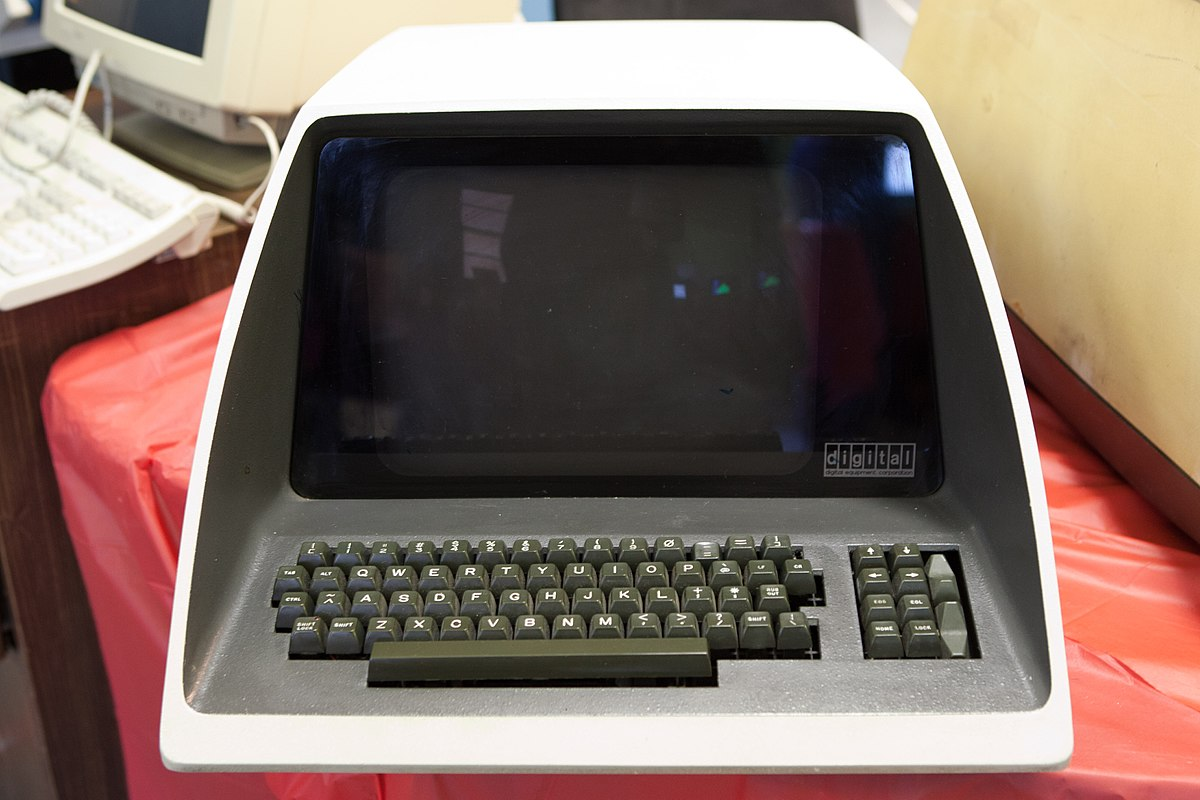
\includegraphics[width=0.9\textwidth]{5.png}
    \caption{Физический термиал}
    \label{fig:5}
\end{figure}

\begin{figure}[ht]
    \centering
    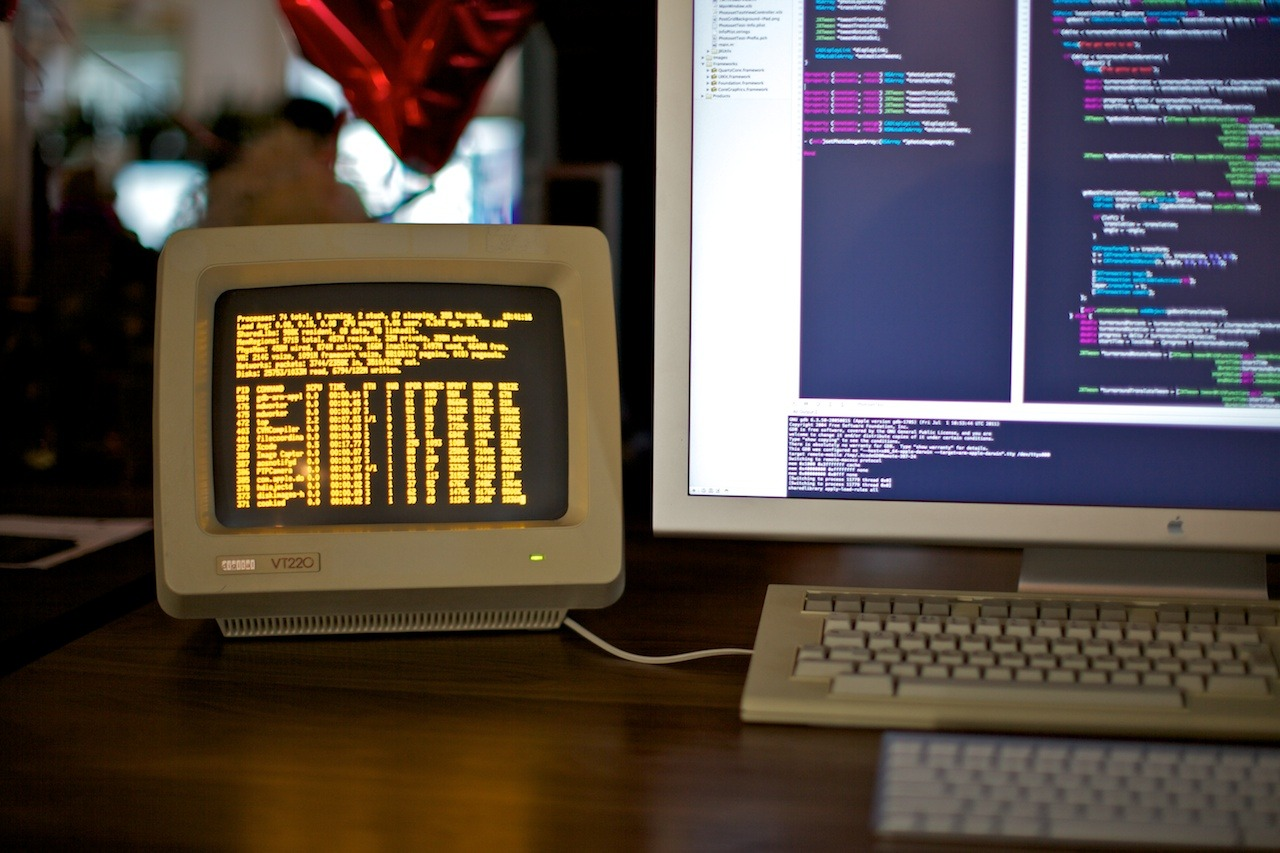
\includegraphics[width=0.9\textwidth]{6.png}
    \caption{Физический термиал}
    \label{fig:6}
\end{figure}

Логин в Linux не имеет значения для самой ОС, система ориентируется по UID (User Identificator), 
который принимает значение от $2$ до  $2^{32} - 1 $. Именно UID определяет права пользователя.
UID root = 0

\textit{Шебанг (Shebang) } --- это комбинация bash \# и bang ! за которым следует путь оболочки bash. 
Это первая строка скрипта. Шебанг говорит оболочке выполнить его через оболочку bash.
Если присутствует первая строка \textit{\#!/bin/bash} в файле, такой файл можно запустить 
просто командой \textit{./file}. Иначе придётся явно указывать интерпретатор, то есть
\textit{/bin/bash ./file}


\section{Операционные системы}

\subsection{Ядро ОС}

\textit{Ядро ОС} – центральная часть ОС, обеспечивающая приложениям 
координированный доступ к ресурсам комьютера Рис.~\ref{fig:3}. 
В современных ОС приложение не может напрямую обратиться 
к ресурсам комьютера, поэтому приложения обращаются к \textbf{ядру}.

\begin{figure}[ht]
    \centering
    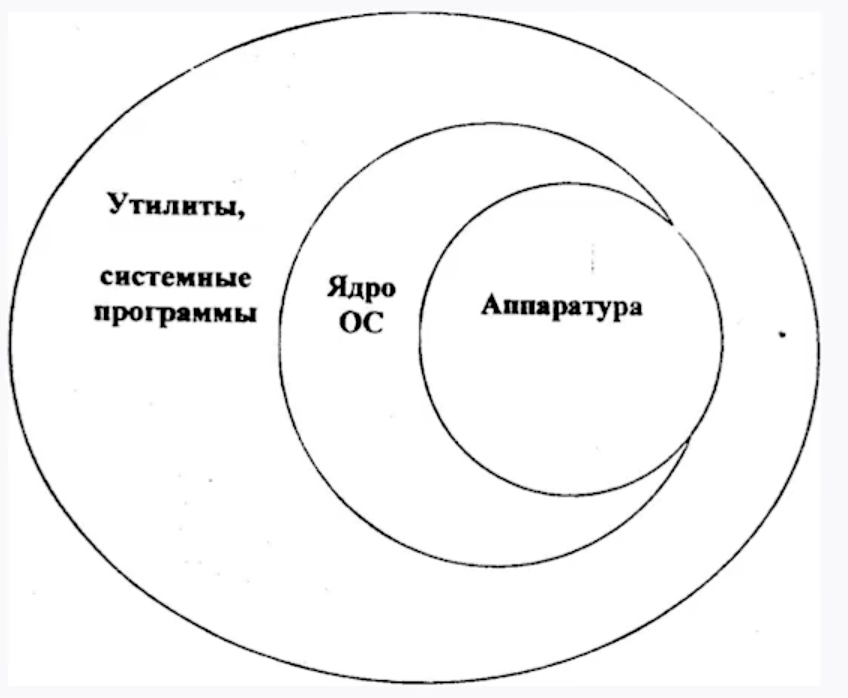
\includegraphics[width=0.5\textwidth]{3.png}
    \caption{Ядро ОС}
    \label{fig:3}
\end{figure}

\textit{Архитектура ядра операционной системы} --- это структура и дизайн основной части операционной системы, которая обеспечивает основные функции управления ресурсами компьютера, планирование выполнения задач, обработку прерываний и обеспечивает взаимодействие между аппаратными устройствами и пользовательскими процессами.

В ОС, основанных на ядре, приложения имеют собственные независимые окружения. То есть
свои участки памяти, своё процессорное время, свой доступ к устройствам 
ввода и вывода.


Современные ОС имеют пространство ядра (где идёт работа с оборудованием)
и пространство пользователя.

\textit{\textbf{Архитектуры ядер}}
\begin{itemize}
    \item Монолитное ядро (самое быстрое) --- Linux
    \item Микроядро (самое отказоустойчивое)
    \item Гибридное ядро --- Windows
\end{itemize}

Ближе к оборудованию --- быстрее, ближе к пространству пользователя --- стабильнее.
(Интересная аналогия: Python, C++, assembler)

\begin{figure}[t]
    \centering
    %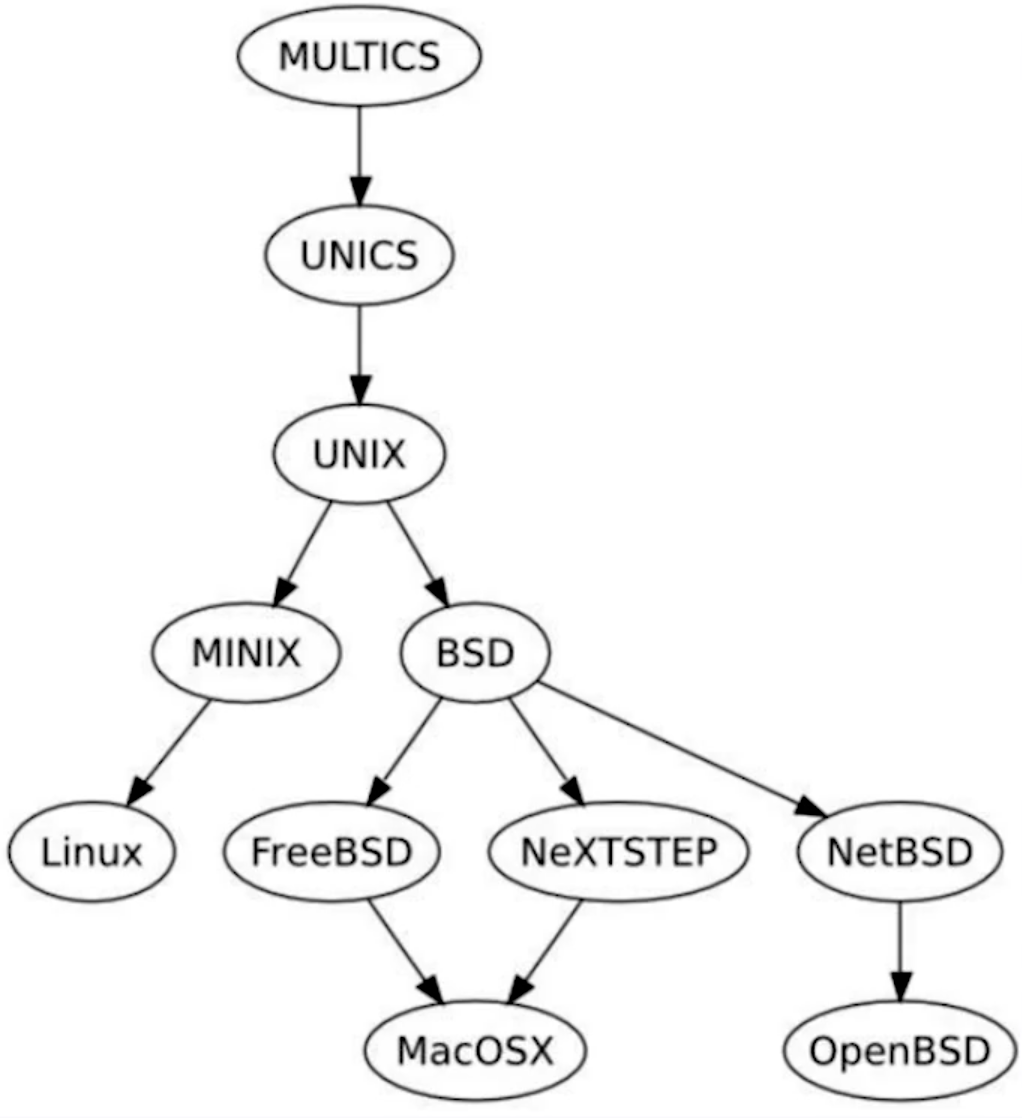
\includegraphics[width=0.2\textwidth]{2.png}
    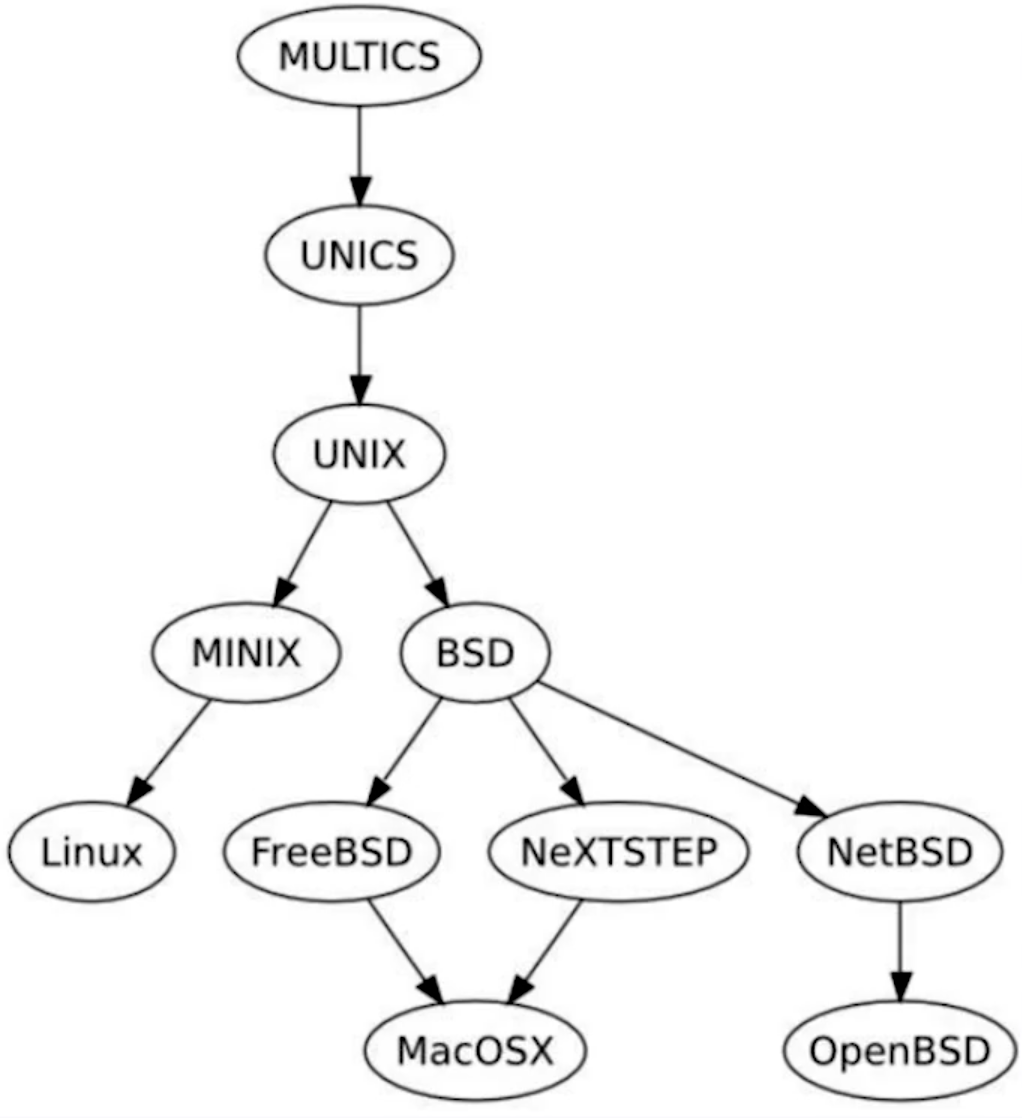
\includegraphics[height=0.3\textheight]{2.png}
    \caption{Развитие операционных систем}
    \label{fig:2}

\end{figure}

Создание ОС с ядром возможно, когда на аппаратном уровне появляются
кольца защиты. (методы разграничения ресурсов компьютера)

\textit{Кольца защиты} --- аппаратная реализация механизма
разграничения ресурсов компьютера 


Интерпретатор команд --- это обычное приложение. В Linux
они бывают разные: \textit{shell, bash, ksh, csh, psh \ldots} Он не 
является частью ядра ОС.

Для Linux не существует расширений файлов, они сделаны 
исключительно для удобства пользователя и для программ, которые 
взаимодействуют с этими файлами

Всё в Unix/Linux --- это файл, просто поток байт

\vspace{\baselineskip} %добавление интервала пустой строчки

\subsection{\textit{UNIX}}

\textit{\textbf{Философия UNX}}
\begin{enumerate}
    \item \textbf{Пишите программы, которые делают что-то одно, но хорошо}
    \item Пишите программы, кототрые работают вместе 
    \item Пишите программы, кототрые поддерживали бы текстовые потоки, так как это универсальный интерфейс
\end{enumerate}

\vspace{\baselineskip} %добавление интервала пустой строчки
 
\textit{POSIX} --- набор стандартов, описывающих 
инетерфейсы между операционной системой и 
прикладной прогаммой (в \textit{UNIX}). (Средство общения 
с ядром ОС). Обеспечивает 
совместимость UNIX-подобных ОС.

Когда разработчики создают программы, используя стандарт POSIX, эти программы могут работать на разных операционных системах без необходимости изменять их код. Это облегчает перенос программного обеспечения с одной системы на другую, так как программы, сделанные в соответствии с POSIX, будут использовать одни и те же команды и функции, доступные во всех системах, поддерживающих этот стандарт.

\textit{POSIX} описывает работу в пространстве пользователя. (видимо, 
именно из-за этого команды в терминалах MacOS, Unix и Linux совпадают)

Команды вроде ls (список файлов и директорий) и pwd (текущая рабочая директория) являются стандартными командами, определенными в стандарте POSIX.

POSIX определяет интерфейс и поведение для командной оболочки и других системных команд в операционных системах, таких как UNIX, Linux, macOS и другие, чтобы обеспечить переносимость программ между различными системами.

Сейчас UNIX используется в серверах и мейнфреймах

\textit{Мейнфрейм (Mainframe)} --- это тип большого и мощного компьютера, который обычно используется в корпоративных средах для обработки больших объемов данных и критически важных бизнес-приложений.
(Например, используется в центрах усправления (космическими) полётами, в банках, на биржах --- в отраслях, где
важна каждая \textit{наносекунда}). (Используется в критически важных задачах, где
важна скорость и бесперебойность)

На всех суперкопьютерах установлен Linux, потому что они решают сложные математические
задачи, если они вдруг остановятся, ничего критического не произойдёт.






\subsection{Структура каталогов в Linux}

См. Рис.~\ref{fig:4}

Основные каталоги
\begin{itemize}
    \item / --- root
    \item /bin --- Необходимые утилиты, необходимые при работе всем пользователям (и в однопользовательском режиме)
    \item /boot --- загрузочные файлы (файлы загрузчика, ядро, initrd, System.tap)
    \item /dev --- основные файлы устройств
    \item \textbf{/etc} --- общесистемные конфигурационные файлы (настройки) (настройки ОС и служб ОС)
    \item /home --- домашние каталоги пользователей (их персональные настройки и данные)
    \item /lib --- Основные библиотеки, необходимые для работы программ из /bin и /sbin 
    \item /media --- Каталог, где производится монтирование сменных носителей (USB, CD-ROM)
    \item /mnt --- каталог содержит временно монтирование файловые системы 
    \item /opt --- Дополнительные программное обеспечение 
    \item \textbf{/proc} --- каталог, которые содержит информацию о всех процессах в нашей ОС
    \item /root --- домашний каталог пользователя \textit{root}
    \item /run --- информация о системе с момента её загрузки (что запущено и чем это работает)
    \item /sbin --- основные системные исполняемые файлы (основыне программы для настройки и администрирования сисетмы, \textit{init, ifcondif, iptables})
    \item /srv --- данные для серисов, представляемых системой (\textit{www} или \textit{ftp})
    \item \textbf{/sys} --- содержит информацию об устройствах, драйверах и некоторых свойствах ядра
    \item /tmp --- временные файлы
    \item /usr --- Большинство пользовательских приложений и утилит (используемых в многопользовательском режиме)
    \item /var --- изменяемые файлы. (файлы регистрации, временные почтовые файлы, файлы спулеров)
    \item /var/log --- логи
    \item /home/username --- домашний каталог пользователя 
\end{itemize}

\subsection{Установка ПО в Linux}

\textit{Установка ПО в Linux/Unix --- это просто переписывание бинарных файлов}

\textit{пакет} --- скомпилированный бинарный файл и перечень зависимостей

\begin{enumerate}
    \item Из исходных кодов (файлы на языке С) --- \textbf{плохой способ}
     \begin{itemize}
        \item Можно модифицировать и устанавливать без прав администртора
        \item Поиск зависимостей очень долгий (как и сам процесс компиляции)
        \item Нет контроля ПО. (что, какой версии, куда, когда и кто установил --- нет возможности узнать)
        \item Правильнее будет скопиллировать, собрать пакет и пакет установить с помощью пакетоного менеджера (будет вестись запись установленного ПО и версий)
     \end{itemize}
    \item Из пакетов 
    \begin{itemize}
        \item Сразу видны зависимости
        \item Не тратится время на компилляцию 
        \item Просто распаковка архива и копирование файлов в нужное место ОС (если есть все  зависимсти)
        \item Есть контроль версий ПО 
        \item Нужны права администратора 
        \item Пакеты создаются под определённый дистрибутив Linux 
    \end{itemize}
    \item Из репозитория --- \textbf{лучший способ}
    \begin{itemize}
        \item Сразу виден перечень зависимостей 
        \item Есть контроль версий ПО 
        \item Как правило, все зависимости устанавливаются автоматически из репозитория
        \item При установке пакетный менеджер сообщит, что нужно и сколько места это займёт
        \item Репозиторий может быть локально или где-то на серверах
    \end{itemize}
\end{enumerate}

\begin{figure}[ht]
    \centering
    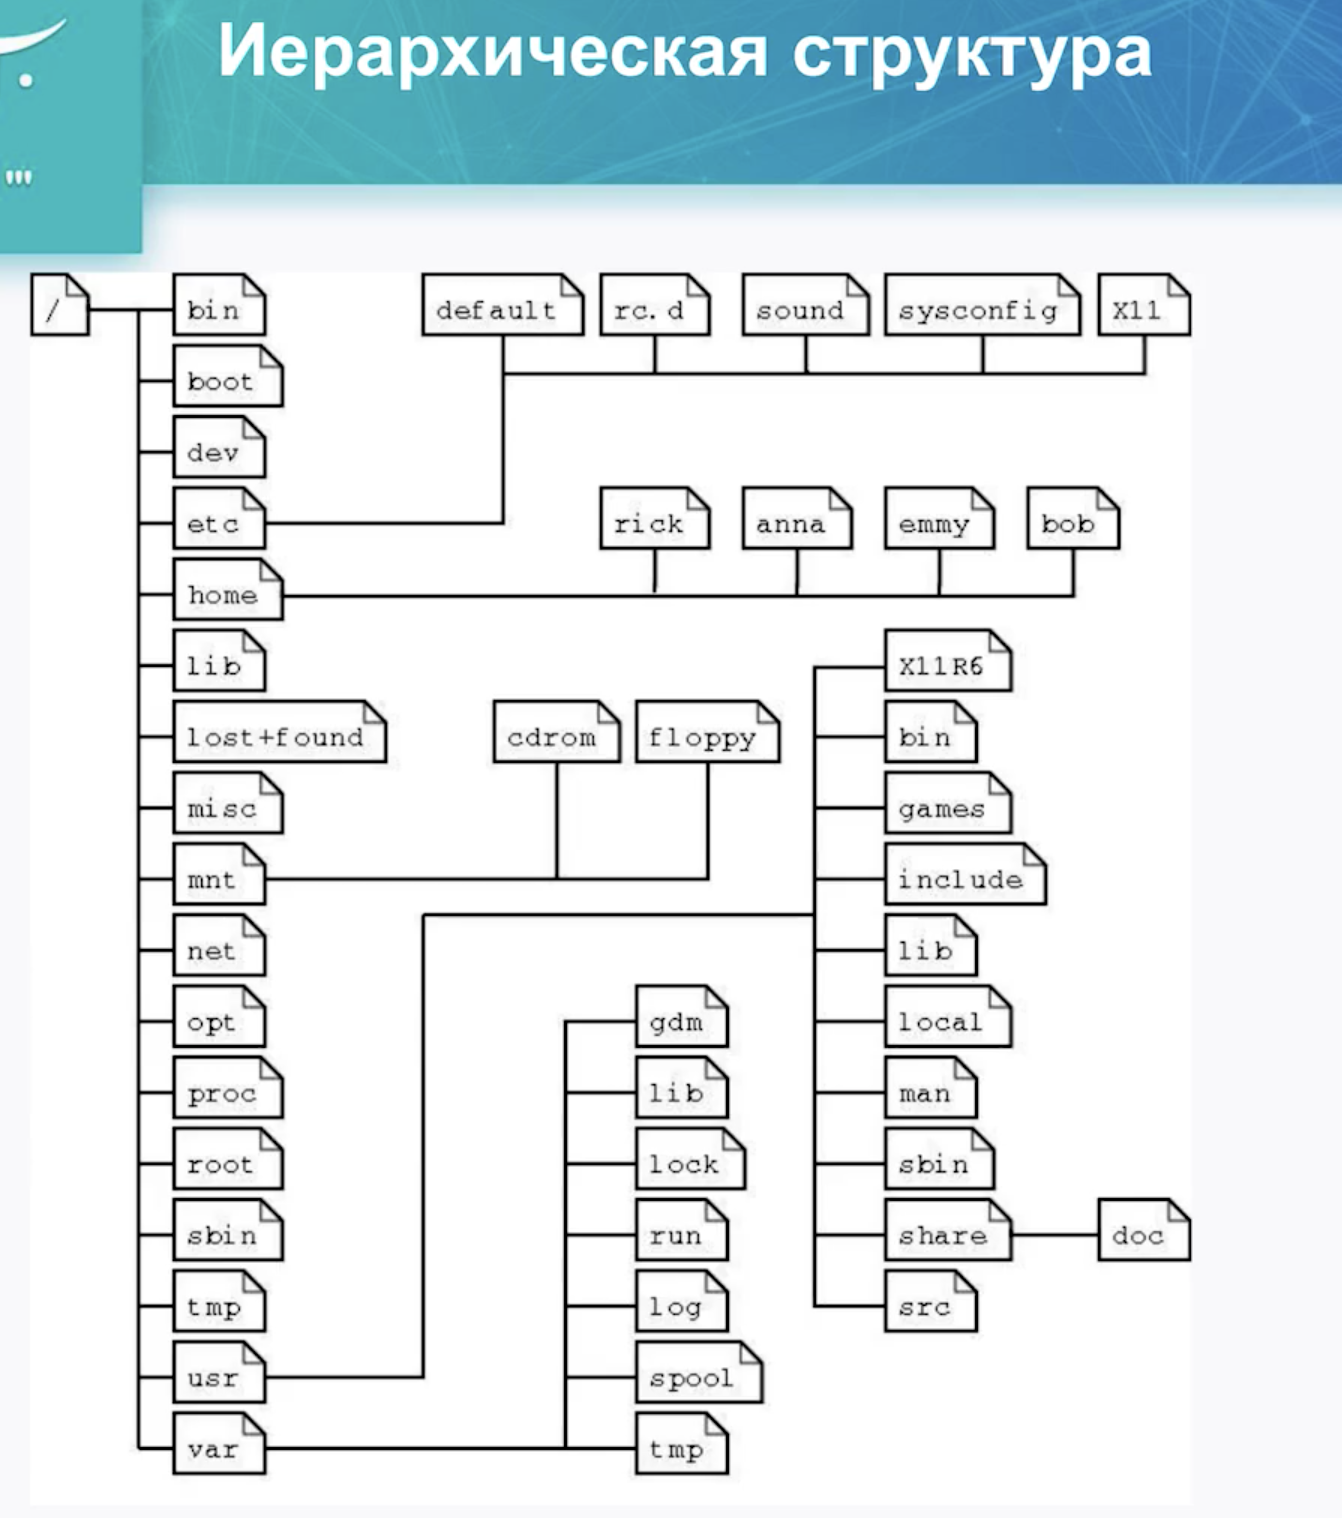
\includegraphics[width=0.6\textwidth]{4.png}
    \caption{Структура каталогов в Linux}
    \label{fig:4}
\end{figure}

\subsection{Создание Linux}
Linus Torvalds в 1991 создал \textit{\textbf{ядро}} операционной системы Linux.
Ядро --- часть ОС, которая отвечает за взаимодействие с оборудованием и предоставляет
определённый интерфейс (в данном случае \textit{POSIX})
Пользователи и администраторы не работают с самим ядром, они работают в пространстве пользователя

У Richard M. Stallman было готово окружение GNU, но не было ядра. 

Проекты объединились и образовалась ОС GNU/Linx. 
OC GNU/Linux --- это ядро и набор программ. 

Официальная версия ядра vanilla kernel \textit{www.kernel.org/}

\vspace{\baselineskip}
\textit{\textbf{Различия дистрибутив}}
\begin{itemize}
    \item Разные версии ядра
    \item Разная структура каталогов
    \item Разные менеджеры пакетов
\end{itemize}


\subsection{Файловые системы}

\textit{FHS} (Filesystem Hierarchy Standard) --- это стандарт иерархии файловой системы для операционных систем на основе Linux. Этот стандарт определяет, как должна быть организована файловая система Linux, чтобы обеспечить единообразие и совместимость между различными дистрибутивами Linux.

\textit{FHS} определяет структуру каталогов и расположение основных системных файлов и приложений на файловой системе Linux. Он определяет, куда должны быть установлены различные типы файлов, какие каталоги являются общими для всех пользователей, какие - системными, а также какие каталоги являются временными, для данных приложений и так далее.

Стандарт FHS обеспечивает стабильность и портируемость между различными дистрибутивами Linux, что позволяет разработчикам программного обеспечения и администраторам системы создавать и управлять приложениями с минимальными проблемами совместимости.

В Linux достаточно часто используются файловые системы типа ext (ext2, ext3, ext4).
Минимальная единица хранения информации на диске --- блок. 

В Linux и других Unix-подобных операционных системах, inod (или инод, inode) представляет собой структуру данных, используемую для хранения метаданных о файлах в файловой системе. Inode (инод) хранит информацию о файле, такую как разрешения доступа, владелец, временные метки (время создания, доступа и модификации), размер файла, количество жестких ссылок и местоположение данных файла на диске.

Когда вы создаете новый файл, операционная система резервирует для него соответствующий inode, который хранит информацию о файле. Каждый inode имеет уникальный номер, который идентифицирует файл внутри файловой системы.

Когда вы выполняете различные операции с файлами (читаете, записываете, изменяете права доступа и т.д.), операционная система использует информацию из inod для обработки этих операций.

Посмотреть индоды можно командой \$ ls -li или \$ stat file

Каталог --- представляет собой соответсвие имён файлов и их инод. Имя каталога хранится в самом каталоге.

\vspace{\baselineskip}
При удалении файла просто удаляется его имя из каталога. Удаляется вся информация
о месторасполажении файла, удаляется его инода. Вручную восстановить данные можно (найти 
эти данные на диски и убедиться, что это именно они). Но утилиту для восстановления написать невозможно, 
потому что после удаления инода не будем ничем отличаться от никогда не используемой иноды.
(по крайней мере для файловой системы ext4).

Каталог и директория являются \textit{синонимами}

\subsection{Hardlink и Softlink}

\textbf{Hardlink}

\textit{Hardlink} --- это ещё одна запись в каталоге о файле. В выводе утилиты ls -l во втором
столбце мы видим количество hardlink для этого файла.

Для создания hardlink есть утилита \$ ln \textit{что куда}
То есть 

\$ ln file1 file3 --- file3 это ссылка на file1

$ \Rightarrow $ файл существует до тех пор, пока $ \exists $ хотя бы один hardlink на него.

\textbf{То есть при удалении одного hardlink (одной ссылки на файл) с самим файлом ничего не произойдёт.}
Все созданные hardlink равноправны. Нет главного hardlink

\vspace*{\baselineskip}

\textbf{hardlink нельзя создавать на каталоги!}

\textbf{hardlink можно создавать только в пределах одного диска, одной файловой системе}. 
Потому что иноды уникальны только в рамках одного диска.

\vspace*{\baselineskip}

\textbf{Softlink}

Это обычные ярлыки (как в Windows)
То есть это файлы, которые содержат с себе ссылку на другой файл.

\$ ln \textbf{-s} file1 file3

У Softlink права 777 (но, если перейти к файлу, на который ведёт ссылка, вступят в силу его права)

В выводе ls -l первая буква в правах у softlink --- l

\textbf{Softlink можно создавать на каталоги и между разными файловыми системами (дисками)}

Чаще используются Softlink. 

\textbf{Пример:} если вышло обновление java, можно не переписывать путь к новой java в всех программах, которые 
её исползуют. Можно просто создать один softlink java, который будет смотреть на нужную версию java.


\subsection{Работа с файлами}

\textbf{grep}

\$ grep \textit{шаблон путь}

\$ grep "Failed" \hspace{0.1cm} ./log

\$ grep -i --- вне зависимости от регистра шаблона

\vspace*{\baselineskip}

\textbf{head}

\$ head~./ log --- вывод первых 10 строк файла

\$ head -3 ~ ./ log --- вывод первых 3 строк файла (или \$ head -n 3 --- рекомендуется так)

\vspace*{\baselineskip}

\textbf{tail}

\$ tail ./log --- последние 10 строк файла

\$ tail -n 3 ./log 

\textbf{важный ключ -f} --- продолжит в режиме реального времени выводить строки, если 
они будут добавляться

\$ tail -f ./log 

\vspace*{\baselineskip}

\textbf{more}

\$ more file --- просмотр файла (можно пролистывать файлы)

\vspace*{\baselineskip}

\textbf{less}

\$ less file --- просмотр файла (можно пролистывать стрелочками)

если нажать / --- откроется поиск по файлу

\subsection{Потоки}
\$ ls -i file1 2> file2 --- перенаправим поток ошибок в файл file2

\$ ls -li file1 2> file2 1>file3 --- ещё и поток вывода (1) перенаправим в file3 одной командой

При этом $>>$ добавляет информацию в файл, а $>$ перезаписывает файл целиком

\textbf{Команды в \textit{bash} выполняются справа налево}

\$ tail -n 50 log > log --- в log ничего не будет, так как сначала будет проверено, что файл существует, 
затем из-за $>$ он будет обнулём. И только потом будет вывод файла

\textbf{Pipe (Конвейер) |}

\$ ls -li file1 | grep \^ \-- (применяем утилиту и перенаправляем её вывод в утилиту grep, которая 
выводит только те файлы, которые начинаются (из за галочки)  с символа \--)

Чтобы вывести информацию и на экран и в стандартный поток вывода

\$ ls -l | tee file

\$ ls -l | tee -a file --- чтобы не перезаписывать, а добавит информацию в файл

Альтернатива этому --- перенаправлять вывод команды в файл, а в другом окне 
терминала читать этот файл с командой \$ tail -f

\$ ls -l file 1>file2 2 $>$ \&1 --- поток 2 направляется туда же, куда и поток 1

\& --- адрес чего-либо

Всё, что направлено в поток /dev/null --- уходит в <<Чёрную дыру>>

\subsection{Условия}

\textit{Интересный факт:} в bash \textit{True} --- это 0 (а не 1), а не 0 --- \textit{False}

\$ echo \$? --- (\$ --- обозначение переменной, а ? --- код возврата последней команды). То есть таким образом
мы можем посмотреть код возврата последней команды

\textbf{\&\& --- оператор И}

\textbf{|| --- оператор ИЛИ}

\textbf{; --- оператор НЕ ИМЕЕТ ЗНАЧЕНИЯ}

command1 ; command2 --- command2 будет выполнена вне зависимости от кода возврата command1

\subsection{Диски и монтирование}
Диски находятся в специальном каталоге /dev

sda, sdb  и тд --- это физические диски

sda1, sdb2 --- (с цифрами) это логические диски

\textbf{VFS Virtual File System} --- программный интерфейс между ядром и драйвером конкретной
файловой системы

Монтирование --- связь VFS с реальной файловой системой

Какой диск куда смонтирован можно посмотреть через утилиту df -h (-h чтобы в GiB был размер)

Для монтирования используются команды \textit{mount} и \textit{unmount}



\section{Полезные bash-команды}

Формат:

\textbf{команда} \textit{ключи} \textbf{\textit{аргументы}}

\vspace{\baselineskip}

\$ man cmd --- более подробная документация, чем в \--\--help

\$ man -k word –– \textit{ищёт в документации ключевое слово word}

\$ uname --- выводит информацию о версии ядра

\$ date --- выводит текущую дату и время

\$ ls -l --- более подробный ls

(Если в первой колонке вывода \$ \textit{ls -l} стоит \textbf{-}, то это файл. А если \textbf{d} --- то директория)

\$ ls -la (или -l -a) --- посмотреть скрытые файлы (имя начинаются с .~)

\$ ls -la .. --- содержимое родительского каталога

\$ \textit{comand} \--\--help --- справочная информация

\$ touch \textit{existing\_file} --- изменить время создания файла

\$ mkdir -p dir1/dir2/dir3 --- рекурсивное создание директорий

Двойное нажатие TAB выдаст спсиок возможных дополнений. Кроме того, если дополнение единственное, 
будет дополено автоматически

\$ cd --- переводит в домашную директорию пользователя (аналог cd \textasciitilde).

Конструкция \$ cd alex эквивалентна \$ cd ./alex

\vspace{\baselineskip}
\textbf{Маски для файлов (<<Регулярные выражения>>)}

* --- любой набор любых символов

? --- один любой символ

\$ rm *2 --- (всё, что оканчивается на 2)

\$ rm file* --- (всё, что начинается с file)

\$ rm *.pdf --- (все pdf файлы)

\$ rm garbadge.*

\vspace{\baselineskip}

\$ rmdir \textit{dir1} --- удаление \textbf{пустой} директории

\$ cp -r dir1 dir2 --- рекурсивное копирование директории и всего её содержимого
(из директории dir1 в dir2)

При этом

\$ mv dir1 dir2 --- перемещение директори (работает без ключей)

\vspace{\baselineskip}

\$ type \textit{command} --- выводит сведения о команде (внутренняя --- принадлежит ОС,
или внешняя --- просто исполняемый файл (в Linux большинство команд именно такие))

\textbf{Пример}

\$ type cd 

cd is a shell builtin --- команда встроена в оболочку

\$ type cp

cp is /bin/cp --- просто исполняемый файл (как и mv, rm \dots)

\$ type ls

ls is aliased to `ls --color=auto'

\vspace{\baselineskip}

\$ which \textit{cmd} --- показывает путь к бинарному файлу \textit{cmd}

Пример

\$ which ls

/bin/ls

\vspace{\baselineskip}

\$ who --- кто сейчас работет на этом сервере, к какому терминалу он подключен, 
когда он подключился и с какого адреса

\textbf{Пример}

\$ who

ubuntu   pts/0        2023-07-26 09:53 (192.168.64.1)

ubuntu   pts/1        2023-07-26 09:55 (192.168.64.1)

\$ (\textit{MacOS}) who

alexey           console      24 июл 08:14 

alexey           ttys002      26 июл 09:51 

\vspace{\baselineskip}


\$ id \textit{user} --- информация о пользователе

\$ chmod u-w --- убирает права на запись для пользователя

(u --- user, g --- group, o --- others, a --- all, \--- --- убрать, + --- добавить)

\$ chmod u+rwx, g-x+rw, o-rwx file

\% chmod a+rwx file --- дать всем полные права

\$ chmod +x file --- сделать исполняемым для псех (эквивалентно chmod a+x file)

Внимание: если изменить права для директории, они не изменятся для содержимого директории
для этого нужно использовать \--R (R --- заглавная!)

Информация о дисках

\$ df или \$ df -i

\vspace*{\baselineskip}

\$ hostname -I --- получить IP этой машины

\$ which prog --- узнать, где расположена программа prog

\vspace*{\baselineskip}


\subsection{Работа с пакетами}

\subsection*{Разница между apt и apt-get}
В целом, <<apt>> обеспечивает более современный и удобный подход к управлению пакетами, и его рекомендуется использовать в новых версиях дистрибутивов Ubuntu и других дистрибутивов Debian. <<apt-get>> по-прежнему доступен и может быть полезен в старых версиях или в определенных сценариях, но его использование становится все более устаревшим.

<<apt>> является более современным и дружелюбным к пользователю интерфейсом. Он предоставляет сокращенные команды, такие как <<apt install>> или <<apt remove>> (без приписки \--get), и обеспечивает интерактивную обратную связь с пользователем при выполнении операций.




\subsubsection*{Apt-get}

\$ sudo apt-get update --- обновляет \textit{список пакетов}

\$ sudo apt-get update --- обновляет список и сами \textit{установленные пакеты}

\$ apt-get remove [ \--\--purge ] package --- Если \--\--purge указан, удаляются и конфигурационные файлы.

\subsubsection{Apt}

Инструкция по работе с пакетами от \href{https://losst.pro/kak-polzovatsya-apt}{losst.pro}

https://losst.pro/kak-polzovatsya-apt 

\vspace*{\baselineskip}

\$ sudo apt update --- для обновления кеша пакетов (какие пакеты вообще есть)

\$ sudo apt list --upgradable --- для каких пакетов доступны обновления

\$ sudo apt list --installed --- установленные пакеты

\$ sudo apt full-upgrade --- обновить все пакеты

\$ sudo apt install gimp --- установка пакета

\$ apt download gimp --- скачать deb пакет в текущую папку без установки

Скачивать пакеты надо от имени обычного пользователя, иначе тогда они не будут доступны для работы с ними. Если вам нужно установить пакет из файла, просто передайте путь к файлу команде install:

\$ sudo apt install package --- установка пакета

\$ sudo apt remove package --- для удаления пакета (без конфигурационных файлов)

\$ sudo apt purge package --- для удаления пакета и всех его данных

\$ sudo apt autoremove --- удаление неиспользуемых пакетов

\vspace*{\baselineskip}

\textbf{А что если ввести в терминал команду}

\$ apt moo

\subsection{Пример сборки кода из исходников}


%код
%\begin{lstlisting}
%here we can write some code
%\end{lstlisting}
    

\$ git clone https:/github.com/the-tcpdump-qroup/tcpdump.qit

\$ cd tcpdump

\$ ./confiqure

\$ make

\$ sudo make install

\vspace*{\baselineskip}

Подробная \href{https://habr.com/ru/articles/321468/}{статья} статья по сборке пакетов и по установке из исходников

https://habr.com/ru/articles/321468/


%\subsection{Зависимости}

%\begin{table}[t]
%    \centering
%    \begin{tabular}{|c|c|}
%    \hline
%    Wants & Модули, которые должны быть активированы одновременно,\\ 
%    & если это возможно, но не обязательно \\
%    \hline
%    Requires & Строгие зависимости; отказ от каких-либо предварительных условий \\ 
%    &прекращает работу этой службы \\
%    \hline
%    Requisite & Аналогично \textit{Requires}, но модуль должен быть активным \\
%    \hline
%    BindsTo & Аналогично \textit{Requires}, но модуль должен быть связан еще более тесно \\
%    \hline
%    PartOf & Аналогично Requires, но влияет только на запуск и остановку \\
%    \hline
%    Сonf1iсts & Отрицательные зависимости; не может взаимодействовать \\ &
%    с этими единицами \\
%    \hline
%    \end{tabular}
%    \caption{Явные зависимости}
%\end{table}

\section{Ответы на важные вопросы}

\textbf{Что такое процес в Linux?}

Программа --- это исполняемый файл, который может быть запущен в операционной системе, и когда программа запускается, операционная система создает \textbf{процесс}, который представляет эту работающую программу.

Каждый процесс имеет свой собственный уникальный идентификатор (PID), который используется для управления и отслеживания процессов операционной системой.

Процессы могут быть запущены как фоновые задачи, которые работают в фоновом режиме без взаимодействия с пользователем, или как интерактивные задачи, которые требуют ввода и вывода с помощью терминала или графического интерфейса пользователя.

Каждый процесс имеет свою собственную память и ресурсы, которые используются во время его выполнения.

\vspace*{\baselineskip}

\textbf{Переменные окружения и для чего они нужны}


В контексте Linux окружение --- это набор переменных окружения и их значений, которые определяют поведение и конфигурацию среды выполнения для запущенных процессов. 

Переменные окружения в операционной системе (в том числе в Linux) представляют собой именованные значения, которые определяют окружение, в котором работают запущенные процессы. Эти переменные содержат информацию о системе, пользовательских настройках, путях к исполняемым файлам и другую важную информацию.

\vspace{\baselineskip}

\textbf{Некоторые из распространенных переменных окружения в Linux }

\begin{itemize}
    \item PATH: Одна из самых важных переменных окружения. Она содержит список каталогов, в которых операционная система ищет исполняемые файлы, когда вы вызываете команду в терминале. Когда вы вводите команду в терминале, Linux просматривает все каталоги, указанные в переменной PATH, чтобы найти соответствующий исполняемый файл.
    \item HOME: Указывает домашний каталог текущего пользователя. Когда пользователь входит в систему, его домашний каталог становится текущим рабочим каталогом.
    \item USER и USERNAME: Имя текущего пользователя
    \item TMP или TMPDIR: Указывает каталог для временных файлов, используемых различными программами.
    \item SHELL: Путь к интерпретатору командной строки (shell), используемому по умолчанию для текущего пользователя.
    \item PS1 и PS2: Определяют строку приглашения командной строки (prompt), которая отображается перед вводом команды (PS1) и при продолжении многострочной команды (PS2).
\end{itemize}

\vspace*{\baselineskip}

\textbf{Как программа ищет библиотеку в момент запуска?}

На порядок поиска могут влиять переменные окружения и настройки системы. Но в целом он такой:

\begin{enumerate}
    \item Исходные каталоги программы: Если библиотеки, требуемые программой, находятся в том же каталоге, что и сам исполняемый файл программы, они будут использоваться в первую очередь.
    \item При запуске программы операционная система заранее знает несколько стандартных каталогов, в которых могут находиться общие библиотеки. Эти пути указаны в переменной окружения LD\_LIBRARY\_PATH. Обычно стандартные пути включают /lib и /usr/lib
    \item Каталоги кэширования: Современные версии Linux используют кэширование динамических библиотек для повышения производительности. Кэш содержит информацию о расположении библиотек в системе. Кэшированные данные хранятся в /etc/ld.so.cache
    \item Каталоги из файла конфигурации /etc/ld.so.conf: Файл /etc/ld.so.conf содержит список дополнительных каталогов, в которых могут находиться общие библиотеки. Если есть изменения в этом файле, обычно требуется запустить команду ldconfig, чтобы обновить кэш библиотек.
    \item Системные пути: Если все остальные пути не дали результатов, операционная система будет искать библиотеки в системных каталогах, таких как /lib и /usr/lib.
\end{enumerate}

Как только требуемая библиотека найдена, она будет загружена в память, и программа сможет использовать функции из этой библиотеки в процессе своего выполнения.

\vspace*{\baselineskip}

\textbf{Порядок запуска программ}

\begin{enumerate}
    \item ОС создает новый процесс для этой программы
    \item ОС загружает исполняемый файл программы в память нового процесса.
    \item ОС начинает разрешать зависимости библиотек, ища соответствующие библиотеки, необходимые для выполнения программы.
    \item Когда требуемая библиотека найдена, операционная система загружает ее в память процесса, который выполняется.
    \item После разрешения всех зависимостей и загрузки библиотек, процесс становится полностью загруженным и готовым к выполнению. Операционная система передает управление программе, и она начинает свое выполнение.
\end{enumerate}


\vspace*{\baselineskip}

\textbf{Чем отличается файл программы от файла библиотеки?}

Файл программы (исполняемый файл): Это файл, который содержит всю информацию и код, необходимые для запуска и выполнения отдельной программы. Когда вы запускаете программу, используется этот файл, чтобы программа могла выполнять свои функции. Файл программы --- это конечный результат всего процесса разработки, и он может быть запущен напрямую.

Файл библиотеки (динамическая или статическая библиотека): Это файл, который содержит функции и код, которые могут быть использованы другими программами. Библиотеки создаются для облегчения повторного использования кода и экономии памяти. Этот файл не является полноценной программой, но предоставляет некоторый функционал, который может быть подключен к другим программам. Библиотеки могут быть использованы множеством программ, чтобы они могли обмениваться кодом между собой и не дублировать его в каждой программе.

\vspace*{\baselineskip}

\textbf{Какие ресурсы нужны программе при запуске и при работе?}


\begin{enumerate}
    \item Центральный процессор (CPU): Программе требуется центральный процессор для выполнения своего кода и обработки данных. Чем более сложные операции выполняет программа, тем больше ресурсов CPU она использует.
    \item Память (RAM): Когда программа запускается, ей нужно занять определенный объем оперативной памяти (RAM) для хранения своего кода, данных и временных результатов. При работе программа может активно использовать память для хранения переменных, стека вызовов и других данных.
    \item Ввод/вывод (I/O) устройства: Программы могут взаимодействовать с внешними устройствами через различные каналы ввода/вывода. Например, программы могут читать и записывать данные на жесткий диск, сеть, клавиатуру, монитор и т. д.
    \item Файловая система: Программам может потребоваться доступ к файлам, чтобы считывать конфигурационные данные, записывать журналы и т. д. Для этого требуются права на чтение и запись в соответствующие файлы и директории.
    \item Графический интерфейс: Если программа имеет графический пользовательский интерфейс (GUI), ей понадобятся ресурсы для отображения окон, кнопок, изображений и других элементов интерфейса.
    \item Cистемные вызовы и библиотеки: Для выполнения различных операций, таких как чтение файлов, создание сетевых соединений и другие, программа может вызывать функции из системных библиотек операционной системы.
\end{enumerate}

\vspace*{\baselineskip}

\textbf{Что такое ld.so.cache ld.config?}

\textbf{ld.so.cache}

ld.so.cache, также известный как <<кэш динамической загрузки>>, это файл-кэш, содержащий информацию о разделяемых библиотеках, доступных на вашей системе. Когда исполняемый файл требует загрузку разделяемой библиотеки, динамический линковщик (ld.so) ищет ее в каталогах, перечисленных в ld.so.cache. Если библиотека найдена в кэше, это уменьшает время поиска, так как системе не нужно искать библиотеку в каждом каталоге из списка.

Путь к файлу ld.so.cache обычно: /etc/ld.so.cache

\textbf{ldconfig}

ldconfig --- это утилита командной строки в Linux, которая служит для обновления кэша динамической загрузки (ld.so.cache) с информацией о разделяемых библиотеках в системе. Это делается для того, чтобы динамический линковщик знал о наличии и расположении новых или обновленных библиотек. 

Когда вы устанавливаете новую разделяемую библиотеку на вашей системе, или изменяете пути к существующим библиотекам, вы можете использовать команду \textit{ sudo ldconfig} для обновления ld.so.cache и применения изменений. Это обновит кэш динамической загрузки (ld.so.cache) с текущим списком разделяемых библиотек на вашей системе.

\vspace*{\baselineskip}

\textbf{Что такое монтирование файловой системы?}

Монтирование файловой системы --- это процесс интеграции (подключения) файловой системы к определенной точке монтирования (mount point) в иерархии файловой системы ОС.

Это позволяет операционной системе обращаться к содержимому этой файловой системы и работать с ней как с обычной директорией на жестком диске или другом устройстве.

Когда файловая система монтируется, содержимое устройства (например, жесткого диска, раздела, сетевого ресурса и т. д.) становится доступным для чтения и записи по указанному пути монтирования.

В операционной системе Linux или Unix команда для монтирования файловой системы имеет общий синтаксис:

\$ sudo mount /dev/sdb6 /mnt/

так мы смонтировали раздел /dev/sdb6 в папку /mnt. 
Ещё можно указать файловую систему подключаемого устройства с помощью ключа -t. 

Посмотреть список всех примонтированных устройств можно просто выполнив \textit{mount} без параметров.

Чтобы размонтировать устройство после использования нужна команда:

\$ sudo umount /dev/sdb6.

\textbf{Примечание:}

В большинстве современных дистрибутивов Linux, флешки и другие съемные устройства автоматически монтируются при их подключении к системе. 

Когда вы подключаете флешку к системе, она обнаруживается операционной системой, и если файловая система на флешке распознается, она автоматически монтируется в какую-то директорию, часто в /media или /mnt.



\subsubsection{Из чего состоит пакет?}

Пакет, как правило, содержит само приложение, в откомпилированном  виде, то есть в виде бинарного файла.

Так же в пакете есть метаинформация, которая представляет собой составленное по определённым правилам описание, которое содержит имя пакета, номер версии и сборки, сведения о разработчике и его мастер-сайте, список файлов, их положение в файловой иерархии, список зависимостей. Также, здесь могу присутствовать установочные и настроечные сценарии, необходимые для развертывания приложения.

Пакет содержит набор действий, выполняемых после установки и сценарий, выполняемый в случае удаления пакета.

\vspace*{\baselineskip}

\textbf{Рассмотрим deb-пакет vs code}

После выполнения команды \textit{sudo apt download code} 
был загружен deb-пакет code.

Внутри пакета лежит бинарный файл debian-binary и два архива: control.tar.xz и data.tar.xz.

В первом лежат бинарные файлы:
control (необходим для установки через dpkg), 
postinst (скрипт, отвечающий за то, что будет выполнено после установки), 
postrm (скрипт, отвечающий за действия после удаления) и prerem (скрипт, который запускается перед удалением). 

Во втором имеется вот такая структура: ./usr/share/. В директории share лежит
множество поддиректорий: appdata, applications, bash-completion, code, mime, pixmaps,
zsh.  При установке пакета файлы из каталога data.tar.xz копируются в аналогичные каталоги в корне системы.

\subsubsection{Что происходит в системе при установке пакета в Linux?}

\begin{enumerate}
    \item \textbf{Поиск пакета:} Когда вы выполняете команду установки пакета (например, apt install <пакет>), система управления пакетами начинает поиск пакета в своих репозиториях.
    \item \textbf{Загрузка пакета:} Если пакет найден, система загружает его из удаленного репозитория в локальный кэш.
    \item \textbf{Проверка зависимостей:} Пакет может зависеть от других пакетов для правильной работы. Перед установкой пакета система управления проверяет наличие всех необходимых зависимостей и может установить их автоматически, если они еще не установлены.
    \item \textbf{Распаковка и копирование файлов:} После того, как пакет и его зависимости загружены, они распаковываются и копируются в соответствующие директории на вашей системе.
    \item \textbf{Настройка пакета:} После копирования файлов некоторые пакеты требуют дополнительной настройки. Это может включать создание конфигурационных файлов, добавление системных сервисов, установку прав доступа и т. д.
    \item \textbf{Обновление кэша:} После установки пакета система управления обновляет информацию о пакетах в своем кэше, чтобы отразить изменения и обеспечить последующую возможность установки обновлений.
\end{enumerate}

\textbf{Помимо этого ещё могут протекать такие процессы как}

\begin{itemize}
    \item Создание и изменение конфигурационных файлов: При установке некоторых пакетов могут создаваться или изменяться конфигурационные файлы. Это может включать параметры, которые определяют поведение программы или службы, или другие настройки, влияющие на работу пакета.
    \item Настройка служб: Пакеты, представляющие службы или демоны, могут быть настроены для автоматического запуска при загрузке системы или предоставления возможности их запуска и остановки через специальные команды.
    \item Создание символических ссылок: Некоторые пакеты создают символические ссылки на свои исполняемые файлы в системных каталогах, чтобы обеспечить доступ к ним из любой директории.
    \item Установка документации: Многие пакеты предоставляют документацию, такую как руководства пользователя или справочные материалы, которые устанавливаются в соответствующие каталоги, чтобы пользователи могли получить информацию о пакете.
    \item Регистрация приложения: В графических окружениях пакеты могут регистрироваться, чтобы появляться в меню приложений и быть доступными для запуска через графический интерфейс.
    \item Предварительная компиляция (для исходных пакетов): В некоторых случаях пакетные менеджеры могут компилировать исходный код программы на лету перед установкой, если предлагаемый пакет является исходным пакетом, а не предварительно скомпилированным.
    \item Обновление динамической базы данных: После установки пакетный менеджер обновляет свою базу данных, чтобы отслеживать установленные пакеты и их версии.
\end{itemize}

\subsubsection{На основании чего система примет решение что пакет не подходит?}

Схема на Рис.~ \ref{fig:основания} на стр.~ \pageref{fig:основания}.

При попытке установить пакет, менеджер пакетов (например, apt, yum, dnf, pacman) анализирует указанные зависимости и требования, чтобы определить, можно ли установить пакет на текущей системе. Если есть проблемы, менеджер пакетов выдаст сообщение об ошибке и не выполнит установку.

\begin{enumerate}
    \item Зависимости: Пакет может быть несовместимым из-за неудовлетворенных зависимостей. Это означает, что для установки или обновления пакета требуются другие пакеты или библиотеки определенных версий. Если эти зависимости не удовлетворены или конфликтуют с другими установленными пакетами, система не даст установить данный пакет.
    \item Версия системы: Некоторые пакеты могут быть предназначены только для определенных версий операционной системы или дистрибутива Linux. Если ваша система не соответствует требованиям по версии, пакет не будет устанавливаться.
    \item Архитектура процессора: Пакеты бывают скомпилированы под определенные архитектуры процессора (например, x86, x86\_64, ARM и т.д.). Если пакет предназначен для другой архитектуры, он не будет работать на вашей системе.
    \item Ограничения безопасности: Некоторые пакеты могут быть отклонены из-за ограничений безопасности, например, если они содержат уязвимости или могут представлять угрозу для системы.
    \item Конфликты с другими пакетами: Если пакет конфликтует с другими установленными пакетами и их версиями, система не разрешит его установку. (сначала может попробовать обновить $\exists$ пакеты)
\end{enumerate}

\begin{figure}
    \centering
    \includegraphics{graph1} % Без расширения .tex
    \caption{Совместимость пакета}
    \label{fig:основания}
\end{figure}



\textit{Для установки конфликтующего пакета можно попробовать использовать виртуальную среду.}

\begin{itemize}
    \item В некоторых случаях пакет может быть установлен без явных ошибок, но он может работать нестабильно или некорректно. Возможно, некоторые функции не будут работать или будут работать неправильно.
    \item Несовместимые или устаревшие пакеты могут содержать уязвимости, которые могут быть использованы злоумышленниками для атаки на вашу систему.
    \item Повреждение системы: Некорректно установленные пакеты могут повредить файловую систему или системные компоненты, что может привести к серьезным проблемам.
\end{itemize}

\subsubsection{Понятия <<testing>>, <<backport>>, <<stable>> и <<unstable>>}

Рис.~\ref{fig:graph2} на стр. \pageref*{fig:graph2}.

В качестве примера можно привести NGWF от комании TexArgos (есть ветки Stable и Testing)
или драйвер openrazer (есть stable и daily (то же что unstable)).

\begin{itemize}

    \item \textbf{Testing}
            \begin{itemize}
            \item Testing-версии пакетов представляют собой последние обновления или новые версии программного обеспечения, которые находятся на стадии тестирования. Это значит, что эти версии еще не считаются полностью стабильными и могут содержать ошибки или проблемы. Они предназначены для тестирования и получения обратной связи от опытных пользователей и разработчиков.
            \end{itemize}
    \item \textbf{Backport (обратная портирование)}
            \begin{itemize}
                \item Backport-версии пакетов представляют собой измененные версии программного обеспечения, которые были адаптированы из более новых версий в старые или стабильные версии Linux. Это делается, чтобы предоставить пользователям доступ к новым функциям или исправлениям без необходимости обновления всей операционной системы. Backport-версии обычно более стабильны, чем testing-версии, но все равно могут потребовать дополнительного тестирования.
            \end{itemize}
    \item \textbf{Stable}
            \begin{itemize}
                \item Stable-версии пакетов считаются надежными и безопасными для использования в производственных средах. Они рекомендуются для обычных пользователей и предпочитаются в случаях, когда стабильность является приоритетом.
            \end{itemize}
    \item \textbf{Unstable}
            \begin{itemize}
                \item Unstable-версии пакетов - это самые свежие и нестабильные версии программного обеспечения, которые находятся в активной стадии разработки. Эти версии могут содержать новые функции и исправления, но они также могут быть менее проверены и более склонны к возникновению ошибок. Unstable-версии обычно предназначены для разработчиков и опытных пользователей, которые хотят следить за новыми возможностями и внесениями в разрабатываемые программы.
            \end{itemize}
            
\end{itemize}

\begin{figure}[ht]
    \centering
    \includegraphics{graph2} % Без расширения .tex
    \caption{Типы ПО}
    \label{fig:graph2}
\end{figure}

\vspace{\baselineskip}

\textbf{Дополнение}

Официальные репозитории Debian разделены на несколько веток. Основная ветка, 
которая включается в каждый дистрибутив --- это main. Здесь содержится только 
свободное программное обеспечение. Но вы можете отредактировать /etc/apt.sources.list и 
добавить ветку contrib, которая содержит программы, зависящие от несвободных 
программ. Также можно добавить ветку non-free, в которой содержаться сами несвободные программы.

После выхода новой версии Debian, репозиторий Testing становится Stable и создается новый репозиторий Testing для следующей версии.

\textbf{Какие ещё ветки бывают?}

\begin{itemize}
    \item Experimental 
    
    Здесь находятся новые и настолько нестабильные пакеты, что они не подходят даже для Unstable. Разработчики предупреждают, что пользователям не нужно использовать пакеты отсюда, они могут быть небезопасными даже для опытных пользователей.

    \item Старый stable
    
    Когда выпущена новая версия Debian, ее репозиторий Testing становиться stable. А предыдущий стабильный репозиторий получает статус old-stable. Его нужно поддерживать, потому что многим пользователям нужно время для обновления, а другие и вовсе не спешат обновлять систему.

    \item Security
    
    Репозиторий Security содержит обновления безопасности для пакетов из репозитория stable и old-stable. Он добавляется во время установки и должен оставаться активным.

    \item StableUpdates
    
    Также как и security, этот репозиторий добавляется автоматически. В его адресе используется текущее кодовое имя дистрибутива, например, stretch-updates. Он помогает компенсировать медленный цикл развития Debian, добавляет новые пакеты для важных программ, например, антивирусов.
\end{itemize}


\begin{figure}[ht]
    \centering
    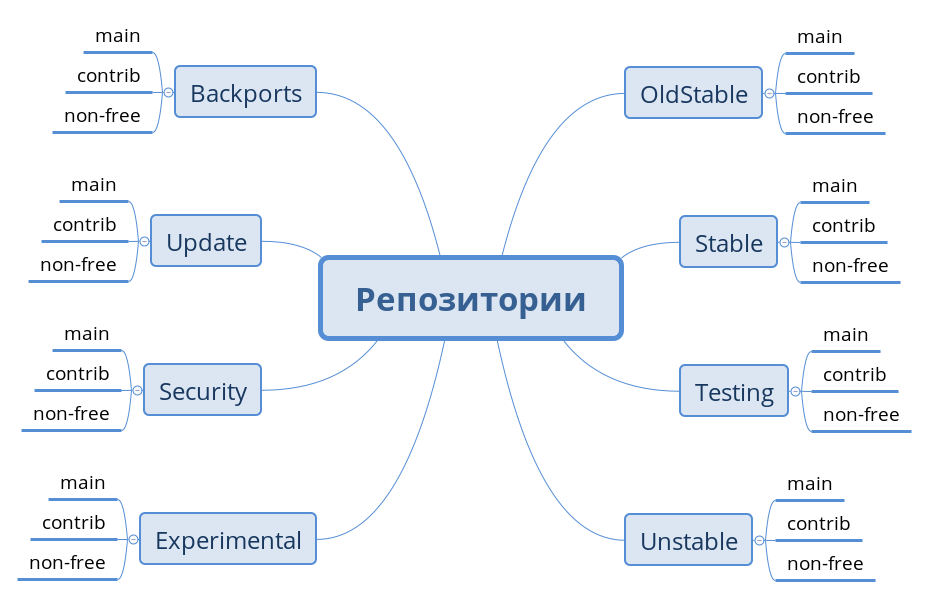
\includegraphics[width=0.9\textwidth]{repos.png} % Без расширения .tex
    \caption{Репозитории}
    \label{fig:repos}
\end{figure}


\end{document}